%% ------------------------------------------------------------------------- %%
\chapter{Resultados}
\label{cap:resultados}

%% ------------------------------------------------------------------------- %%
%% ------------------------------------------------------------------------- %%
\section{Experimentos}
  Os testes foram inspirados pelo estudo de \cite{zagorchev2006comparative}.
A imagem Referência utilizada para os testes foi retirada do software BioImage
\cite{papademetris2005bioimage}, uma ressonância magnética cerebral. A imagem
alvo foi construida aplicando uma função senoidal com diferentes parâmetros
nas três dimensões da imagem referência. A função de deformação escolhida foi:

\begin{align} \label{math:composta}
\begin{split}
  X &= x + 2*sin(\frac{y}{8}) - 2*cos(\frac{z}{16}) \\
  Y &= y + 4*sin(\frac{x}{8}) - 2*sin(\frac{z}{8}) \\
  Z &= z + 2*sin(\frac{x}{16}) - 4*cos(\frac{y}{8})
\end{split}
\end{align}

\begin{figure}[H]
    \centering
    \begin{subfigure}[t]{0.8\textwidth}
      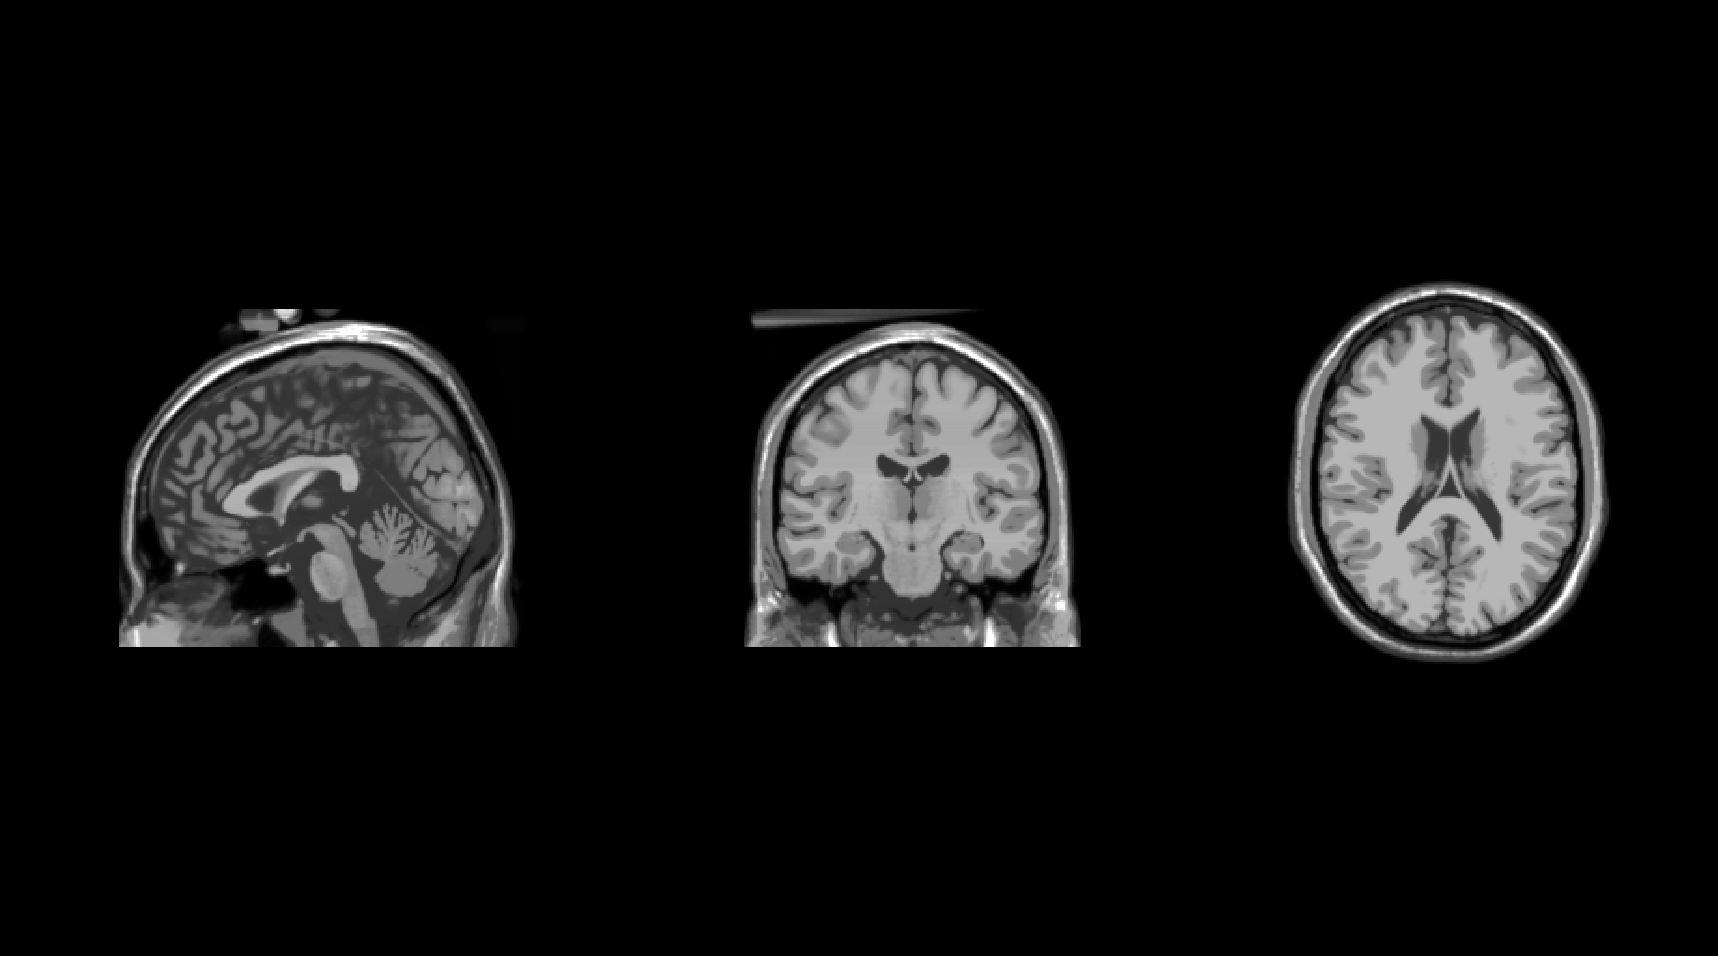
\includegraphics[width=\textwidth]{figuras/referenceImg.png}
      \subcaption*{(a)}
      \label{fig:unequalizedImage}
    \end{subfigure}
    \begin{subfigure}[t]{0.8\textwidth}
      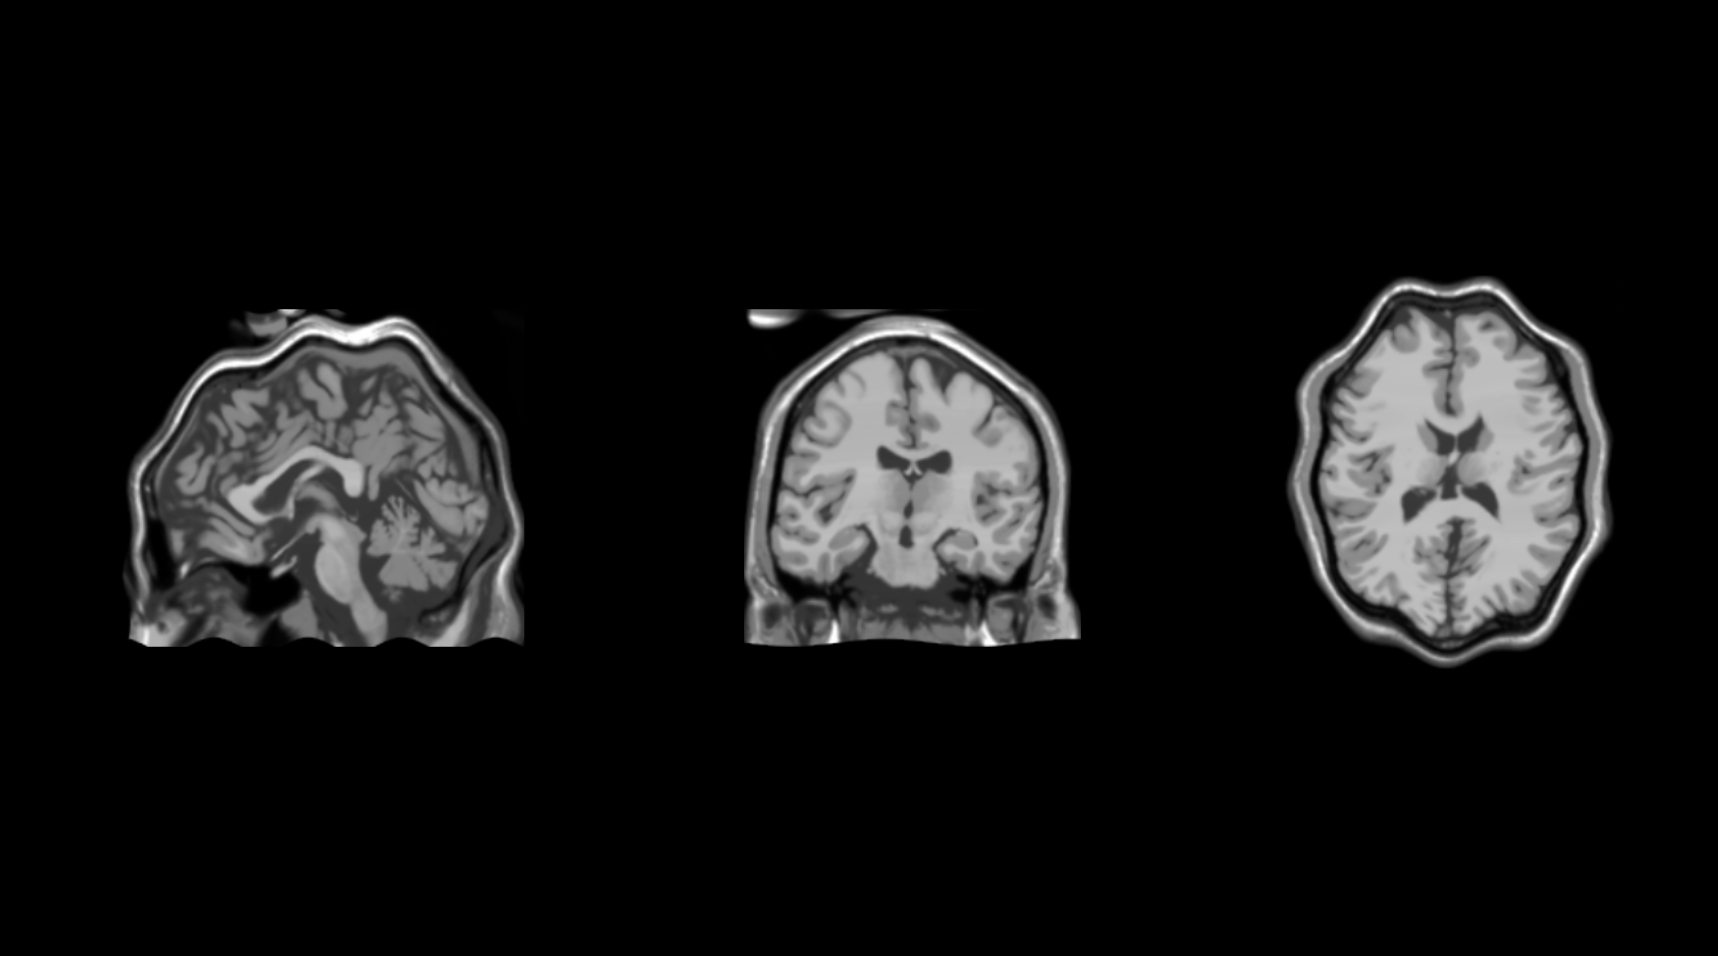
\includegraphics[width=\textwidth]{figuras/targetImg.png}
      \subcaption*{(b)}
      \label{fig:equalizedImage}
    \end{subfigure}
    \source{\cite{papademetris2005bioimage}}
    \caption{Imagens usadas nos testes. A primeira coluna é um corte sagital,
             a segunda coluna um corte coronal e a última um corte axial.
             (a) Imagem referência. (b) Imagem alvo.}
    \label{fig:equalization}
\end{figure}

  A construção artificial das imagens alvo foi escolhida pelos seguintes motivos:
(1) provar a aplicabilidade do algoritmo TPS não é nosso objetivo, (2) com a
função que provocou a deformação em mãos, gerar um conjunto de características
se torna um processo trivial, assim como encontrar as correspondências entre
elas, e (3) a corretude da nossa implementação do TPS é facilmente verificavel.

  Para apurar o ganho de desempenho de cada uma das possiveis modificações
descritas na seção \ref{melhoriaDesempenho}, elas foram implementadas de tal
maneira que elas podem ser ativadas ou desativadas independentemente atráves de
um arquivo de configuração. Logo, nosso casos de teste são:

\begin{enumerate}
  \item Paralelamente em CPU (nosso \textit{guideline})
  \item GPU sem nenhuma das melhorias ativadas
  \item Melhoria de cálculo de Ocupação
  \item Melhoria de textura 3D
  \item Melhoria de execução em paralelo
  \item Todas as combinações de duas melhorias ativas por vez
  \item Todas as melhorias ativas
\end{enumerate}

  Cada teste é composto de quatro execuções do TPS, registrando a mesma imagem
alvo com a mesma imagem referência. As características da imagem referência
são distribuidas uniformemente pelas dimensões da imagem, com um fator que
determina a quantidade de características utilizadas. As características da
imagem alvo são construidas aplicando a função de deformação em cada uma das
características da imagem referência, criando um cenário ideal para a execução
do TPS.

  Os testes foram executados em duas máquinas. A primeira é um notebook com
um processador quadcore Intel i5-3337U @ 1.80GHZ, 6GB de memória, e uma GPU
NVIDIA GeForce GT 730M com 384 cuda cores divididos em 2 multiprocessadores e
2GB de memória dedicada. A segunda máquina é uma máquina virtual, com 4
processadores de 2.3GHz, 8GB de memória, e uma GPU GeForce GTX 980 com 2048
cuda cores divididos em 16 multiprocessadores e 4GB de memória dedicada.

\begin{figure}[H]
    \centering
    \begin{subfigure}[t]{0.5\textwidth}
      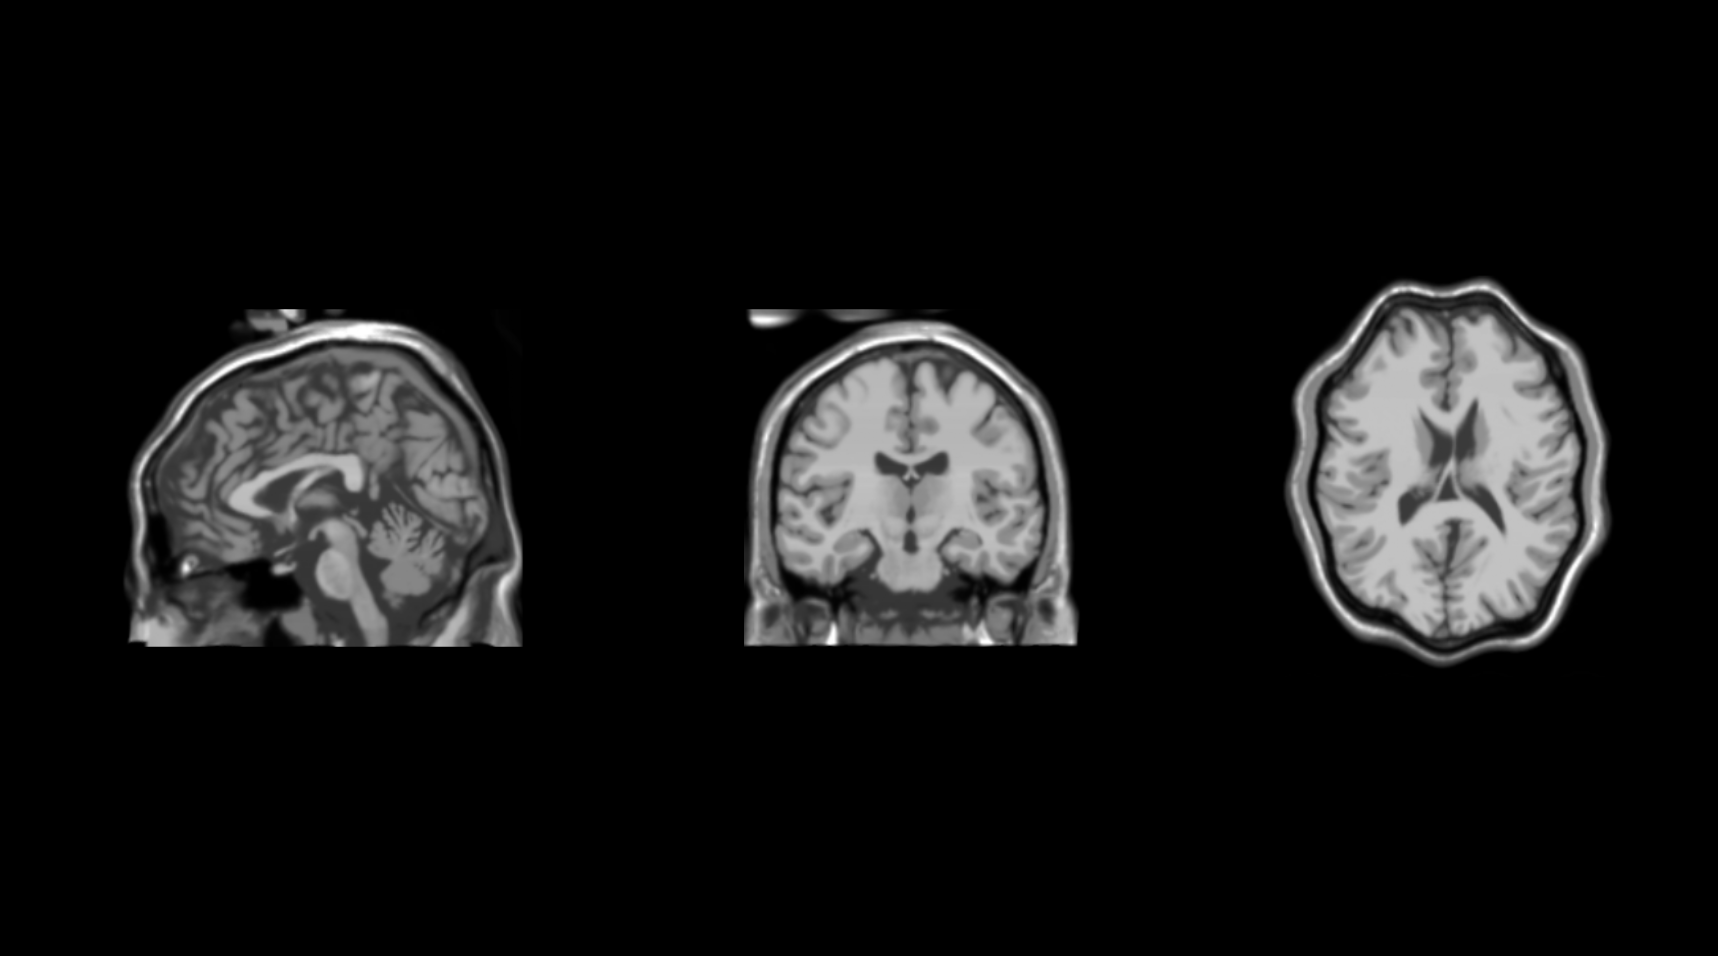
\includegraphics[width=\textwidth]{figuras/result001.png}
      \subcaption*{(a)}
      \label{fig:unequalizedImage}
    \end{subfigure}
    \begin{subfigure}[t]{0.5\textwidth}
      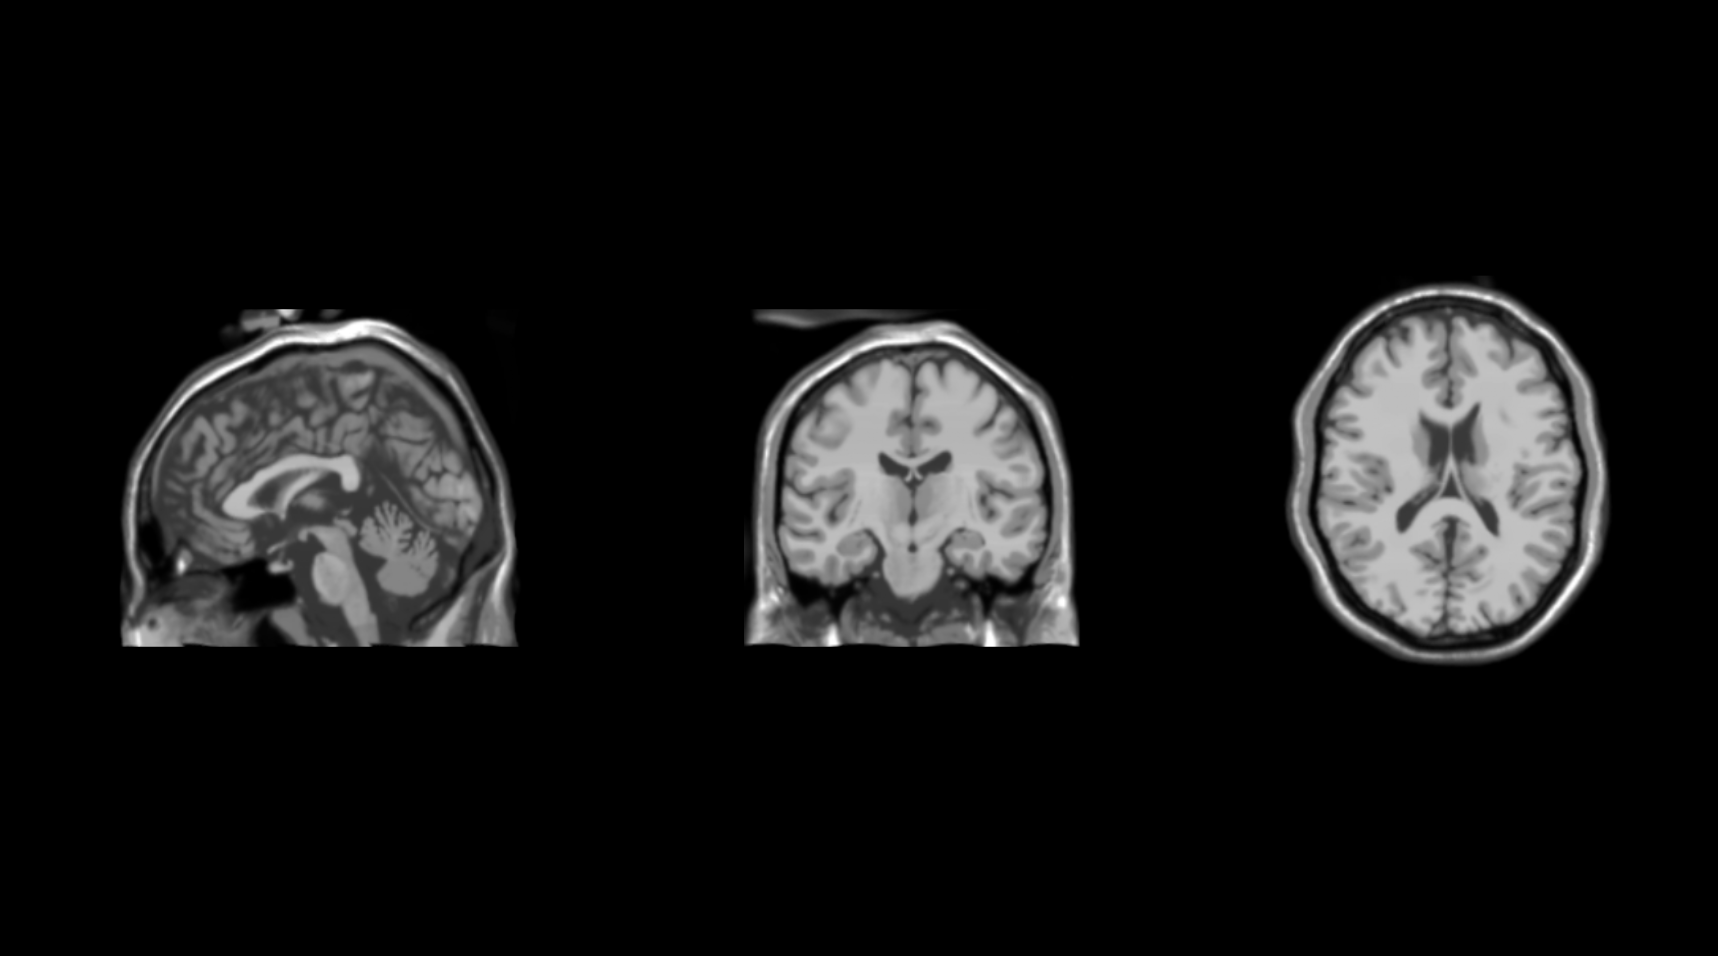
\includegraphics[width=\textwidth]{figuras/result002.png}
      \subcaption*{(b)}
      \label{fig:equalizedImage}
    \end{subfigure}
    \begin{subfigure}[t]{0.5\textwidth}
      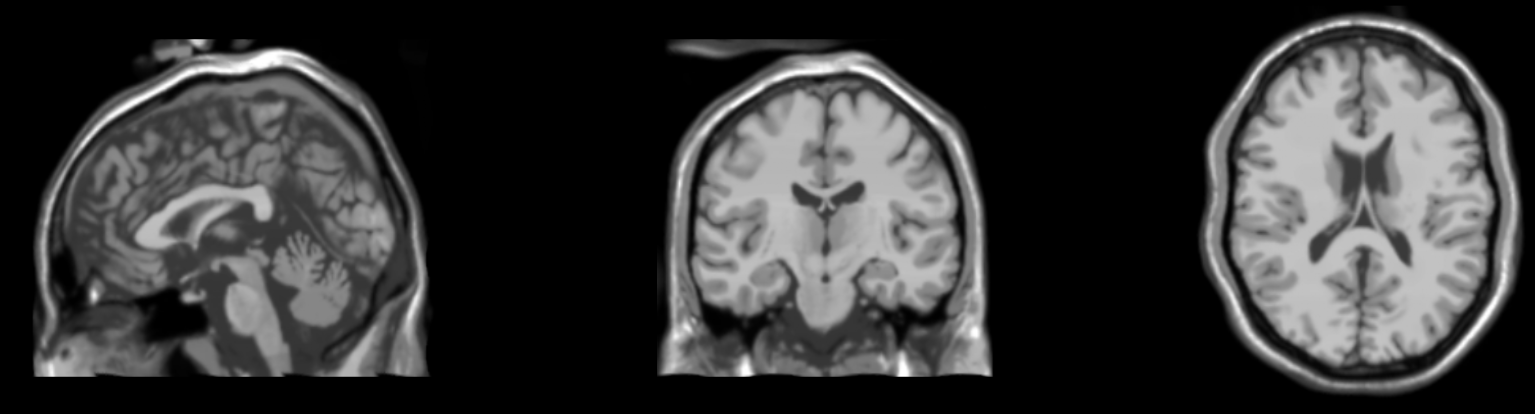
\includegraphics[width=\textwidth]{figuras/result003.png}
      \subcaption*{(c)}
      \label{fig:equalizedImage}
    \end{subfigure}
    \begin{subfigure}[t]{0.5\textwidth}
      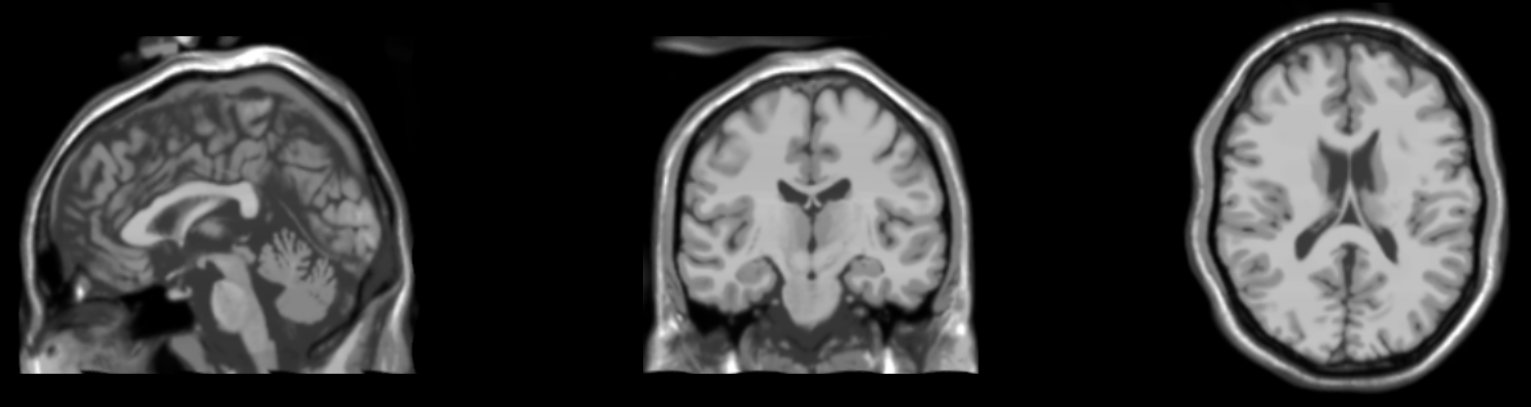
\includegraphics[width=\textwidth]{figuras/result004.png}
      \subcaption*{(d)}
      \label{fig:equalizedImage}
    \end{subfigure}
    \caption{Resultado dos testes. A primeira coluna é um corte sagital,
             a segunda coluna um corte coronal e a última um corte axial.
             (a) Resultado utilizando 576 características.
             (b) Resultado utilizando 2016 características.
             (c) Resultado utilizando 4864 características.
             (d) Resultado utilizando 7942 características.}
    \label{fig:equalization}
\end{figure}
